% Generated by documents/paper/figures/make_rq_appendix.py from the rq02_permutation_null README; do not edit.
\clearpage
\section{Decision accuracy against a no-signal null}
\label{app:rq02_permutation_null}

\begin{rqfinding}
1. \textbf{The benchmark null sits below 0.5.} Pooled over the benchmark tasks, a shuffled proxy scores 0.47--0.49, because proxy ties count as misses. (Figure~\ref{fig:app_rq02_permutation_null}.)

2. \textbf{Few benchmark cells beat their own null.} Only 4--9 \% of the multi-axis benchmark cells (1--2 \% of the mono-axis ones) are above their null at q $<$ 0.05.

3. \textbf{BPB is far above its null.} Per-language BPB reaches 0.79--0.95 against a null of 0.50, and 26--64 \% of its multi-axis cells are significant (2--38 \% mono-axis, where a cell has fewer pairs).
\end{rqfinding}

\paragraph{Question.} How far above chance does a proxy rank the design decisions, once chance is measured cell by cell rather than read off a flat 0.5?

\paragraph{Setup.} Seed-1904 runs of every language setting, ladder and data build, 90M--1.7B, on pairs that may differ on any number of design axes. For every (task, proxy size) cell with at least three comparable pairs, we shuffle the proxy's final scores across the design variants 1000 times and score each shuffle against the unchanged 1.7B ranking with the same sign rule, ties included. A cell's p-value is the share of shuffles that match at least as many pairs, corrected over the cells with the Benjamini-Hochberg procedure. The lines pool the matching pairs over the comparable pairs of the tasks above chance at the proxy and at 1.7B, and the band is the 95\% range of the pooled shuffles. The benchmark line includes the bBPB variants at the sizes where they were computed (175M, 350M and 1B).

\begin{figure}[h]
\centering
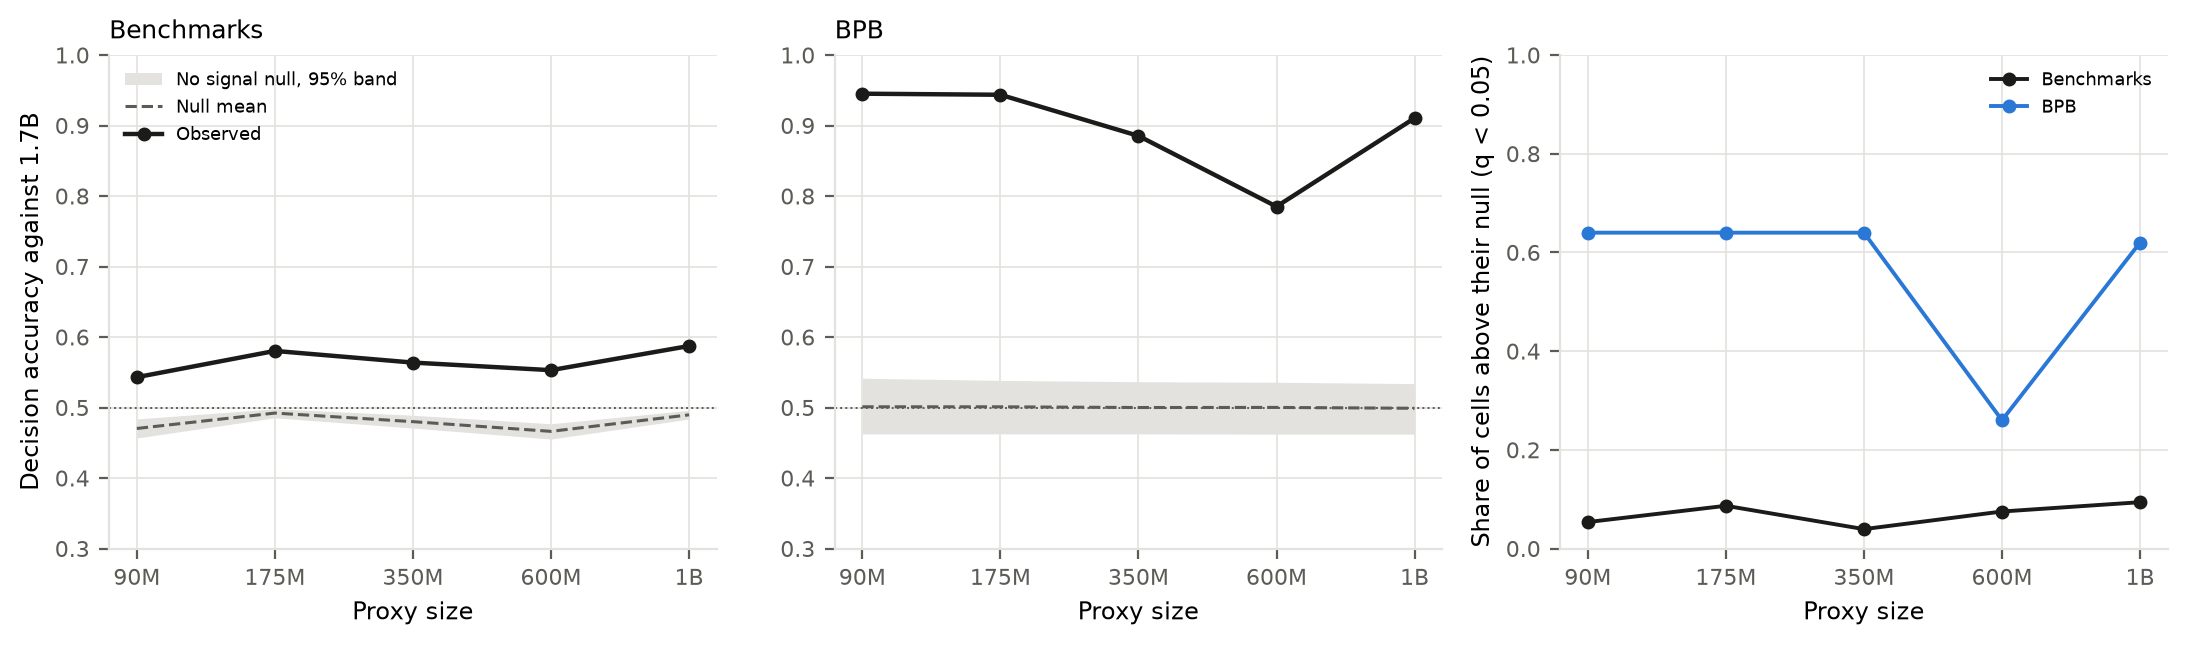
\includegraphics[width=\textwidth]{figures/app_permutation_null.png}
% source: src/signal-and-noise/analysis/rq02_permutation_null/pretraining/predictivity/permutation_null_da_size_paper.png
\caption{DA-size against its no-signal null, multi-axis.}
\label{fig:app_rq02_permutation_null}
\end{figure}
